%%%%%%%%%%%%%%%%%%%%%%%%%%%%%%%%%%%%%%%%%
% Journal Article
% LaTeX Template
% Version 1.3 (9/9/13)
%
% This template has been downloaded from:
% http://www.LaTeXTemplates.com
%
% Original author:
% Frits Wenneker (http://www.howtotex.com)
%
% License:
% CC BY-NC-SA 3.0 (http://creativecommons.org/licenses/by-nc-sa/3.0/)
%
%%%%%%%%%%%%%%%%%%%%%%%%%%%%%%%%%%%%%%%%%

%----------------------------------------------------------------------------------------
%	PACKAGES AND OTHER DOCUMENT CONFIGURATIONS
%----------------------------------------------------------------------------------------

\documentclass[twoside]{article}

\usepackage{lipsum} % Package to generate dummy text throughout this template

\usepackage[sc]{mathpazo} % Use the Palatino font
\usepackage[T1]{fontenc} % Use 8-bit encoding that has 256 glyphs
\usepackage[utf8]{inputenc}
\linespread{1.05} % Line spacing - Palatino needs more space between lines
\usepackage{microtype} % Slightly tweak font spacing for aesthetics
\usepackage{amsmath}

\usepackage[hmarginratio=1:1,top=32mm,columnsep=20pt]{geometry} % Document margins
\usepackage{multicol} % Used for the two-column layout of the document
\usepackage[hang, small,labelfont=bf,up,textfont=it,up]{caption} % Custom captions under/above floats in tables or figures
\usepackage{booktabs} % Horizontal rules in tables
\usepackage{float} % Required for tables and figures in the multi-column environment - they need to be placed in specific locations with the [H] (e.g. \begin{table}[H])
\usepackage{hyperref} % For hyperlinks in the PDF

\usepackage{lettrine} % The lettrine is the first enlarged letter at the beginning of the text
\usepackage{paralist} % Used for the compactitem environment which makes bullet points with less space between them

\usepackage{abstract} % Allows abstract customization
\renewcommand{\abstractnamefont}{\normalfont\bfseries} % Set the "Abstract" text to bold
\renewcommand{\abstracttextfont}{\normalfont\small\itshape} % Set the abstract itself to small italic text

\usepackage{pgf}
\usepackage{tikz}
\usetikzlibrary{arrows,automata}

\newcommand{\rparen}{)}

\usepackage{titlesec} % Allows customization of titles
\renewcommand\thesection{\Roman{section}} % Roman numerals for the sections
\renewcommand{\thesubsection}{\thesection\hspace{1mm}\alph{subsection}}
\titleformat{\section}[block]{\large\scshape\centering}{\thesection}{1em}{} % Change the look of the section titles
\titleformat{\subsection}[block]{\large}{\thesubsection\rparen}{1em}{} % Change the look of the section titles

\usepackage{fancyhdr} % Headers and footers
\pagestyle{fancy} % All pages have headers and footers
\fancyhead{} % Blank out the default header
\fancyfoot{} % Blank out the default footer
\fancyhead[C]{TDT4205 Compilers $\bullet$ Assignment One $\bullet$ \date{\today}} % Custom header text
\fancyfoot[RO,LE]{\thepage} % Custom footer text

%----------------------------------------------------------------------------------------
%	TITLE SECTION
%----------------------------------------------------------------------------------------

\title{\vspace{-15mm}\fontsize{24pt}{10pt}\selectfont\textbf{Theory for Assignment Two}} % Article title

\author{
\large
\textsc{Øyvind Robertsen} \\ % Your name
\normalsize Norwegian University of Science \& Technology \\ % Your institution
\normalsize \href{mailto:oyvinrob@stud.ntnu.no}{oyvinrob@stud.ntnu.no} % Your email address
\vspace{-5mm}
}
\date{}

%----------------------------------------------------------------------------------------

\begin{document}

\maketitle % Insert title

\thispagestyle{fancy} % All pages have headers and footers

%----------------------------------------------------------------------------------------
%	ABSTRACT
%----------------------------------------------------------------------------------------

%\begin{abstract}

%\noindent \lipsum[1] % Dummy abstract text

%\end{abstract}

%----------------------------------------------------------------------------------------
%	ARTICLE CONTENTS
%----------------------------------------------------------------------------------------

\begin{multicols}{2} % Two-column layout throughout the main article text

\section{Problem 1}
\subsection{RE to NFA}

An NFA for the regular expression $R_0 = $ \texttt{(a|b)*c*(d|e)} is shown in figure~\ref{fig:prob1}

\begin{figure}[H]
\centering
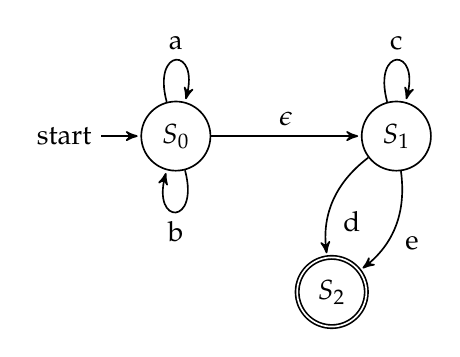
\begin{tikzpicture}[->, >=stealth', shorten >=1pt, auto, node distance=2.8cm,
                    semithick]
    \tikzstyle{every state}=[fill=none, text=black]

    \node[initial, state]   (A)                         {$S_0$};
    \node[state]            (B)     [right of=A]        {$S_1$};
    \node[state, accepting] (C)     [below right of=A]  {$S_2$};

    \path (A) edge [loop above]     node {a}            (A);
    \path (A) edge [loop below]     node {b}            (A);
    \path (A) edge                  node {$\epsilon$}   (B);
    \path (B) edge [loop above]     node {c}            (B);
    \path (B) edge [bend right]     node {d}            (C);
    \path (B) edge [bend left]      node {e}            (C);
\end{tikzpicture}
\caption{Problem 1 NFA} \label{fig:prob1}
\end{figure}

There are many valid NFAs for the RE $R_0$.
This one is (on purpose) rather simple. I could have used Thompsons construction algorithm to recursively create an automaton for each of the subexpressions in $R_0$.
The resulting automaton would however be very large and would not aid in conveying my understanding of automatons.

\subsection{Described language}

The language $L(R_0)$ described by $R_0$ consists of all words ending in either \texttt{d} or \texttt{e}, prefixed by any number (including zero) of \textit{c}s, again prefixed by any number of either \textit{a}s or \textit{b}s.

Examples:

\begin{compactitem}
    \item \texttt{d}
    \item \texttt{e}
    \item \texttt{cd}
    \item \texttt{ce}
    \item \texttt{acd}
    \item \texttt{abcccd}
\end{compactitem}

\subsection{Transition table}

The transition table for the NFA in figure~\ref{fig:prob1} is given in table~\ref{tab:transition-table1}.

\begin{table}[H]
\centering
    \begin{tabular}{l|l|l|l|l|l|l}
    State       & \texttt{a}    & \texttt{b}    & \texttt{c}    & \texttt{d}    & \texttt{e}    & $\epsilon$    \\ \hline
    $S_0$       & $S_0$         & $S_0$         & $\emptyset$   & $\emptyset$   & $\emptyset$   & $S_1$         \\ \hline
    $S_1$       & $\emptyset$   & $\emptyset$   & $\emptyset$   & $S_2$         & $S_2$         & $\emptyset$   \\ \hline
    $S_2$       & $\emptyset$   & $\emptyset$   & $\emptyset$   & $\emptyset$   & $\emptyset$   & $\emptyset$   \\
    \end{tabular}
    \caption{Transition table for the NFA in figure~\ref{fig:prob1}} \label{tab:transition-table1}
\end{table}

\section{Problem 2}

Following the conversion algorithm given in chapter 3.7.1 of the Dragon Book, we create a DFA from the NFA through the following steps.

\begin{figure}[H]
\centering
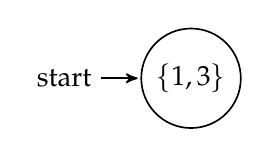
\begin{tikzpicture}[->, >=stealth', shorten >=1pt, auto, node distance=2.8cm,
                    semithick]
    \tikzstyle{every state}=[fill=none, text=black]

    \node[initial, state]   (A)         {$\{ 1, 3 \}$};
\end{tikzpicture}
\caption{Step 1: The initial state of our resulting DFA is given by the $\epsilon$-closure of the initial state of the NFA.} \label{fig:prob2-step1}
\end{figure}


\begin{figure}[H]
\centering
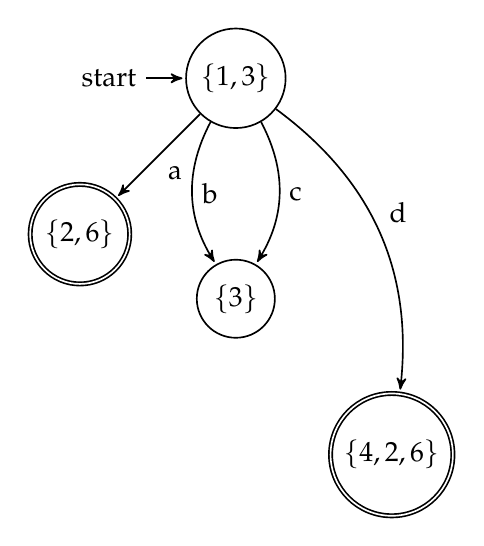
\begin{tikzpicture}[->, >=stealth', shorten >=1pt, auto, node distance=2.8cm,
                    semithick]
    \tikzstyle{every state}=[fill=none, text=black]

    \node[initial, state]   (A)                     {$\{ 1, 3 \}$};
    \node[state, accepting] (B) [below left of=A]   {$\{ 2, 6\}$};
    \node[state]            (C) [below of=A]        {$\{ 3 \}$};
    \node[state, accepting] (D) [below right of=C]  {$\{ 4, 2, 6\}$};

    \path (A) edge                  node {a}            (B);
    \path (A) edge [bend right]     node {b}            (C);
    \path (A) edge [bend left]      node {c}            (C);
    \path (A) edge [bend left]      node {d}            (D);
\end{tikzpicture}
\caption{Step 2: For each symbol in the input alphabet, we compute the $\epsilon$-closure of the set of states reachable from the initial state through the symbol in question.
The resulting symbol-set pairs are added to our DFA\@.
This process is repeated with each added set as the initial set of states until no new sets are added.
Any set of states containing a state that is an accepting state in the NFA, automatically becomes an accepting state in the DFA\@.
This figure shows the result of one such iteration.
}
\label{fig:prob2-step2}
\end{figure}

\begin{figure}[H]
\centering
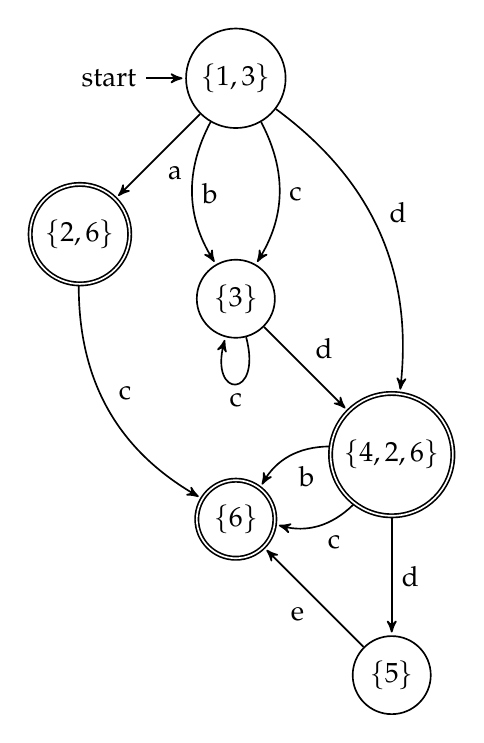
\begin{tikzpicture}[->, >=stealth', shorten >=1pt, auto, node distance=2.8cm,
                    semithick]
    \tikzstyle{every state}=[fill=none, text=black]

    \node[initial, state]   (A)                     {$\{ 1, 3 \}$};
    \node[state, accepting] (B) [below left of=A]   {$\{ 2, 6\}$};
    \node[state]            (C) [below of=A]        {$\{ 3 \}$};
    \node[state, accepting] (D) [below right of=C]  {$\{ 4, 2, 6\}$};
    \node[state, accepting] (E) [below of=C]        {$\{ 6 \}$};
    \node[state]            (F) [below of=D]        {$\{ 5 \}$};

    \path (A) edge                  node {a}            (B);
    \path (A) edge [bend right]     node {b}            (C);
    \path (A) edge [bend left]      node {c}            (C);
    \path (A) edge [bend left]      node {d}            (D);
    \path (C) edge [loop below]     node {c}            (C);
    \path (C) edge                  node {d}            (D);
    \path (B) edge [bend right]     node {c}            (E);
    \path (D) edge [bend right]     node {b}            (E);
    \path (D) edge [bend left]      node {c}            (E);
    \path (D) edge                  node {d}            (F);
    \path (F) edge                  node {e}            (E);
\end{tikzpicture}
\caption{Step 3: The full DFA with states named for the sets of NFA states they represent.} \label{fig:prob2-step3}
\end{figure}

\begin{figure}[H]
\centering
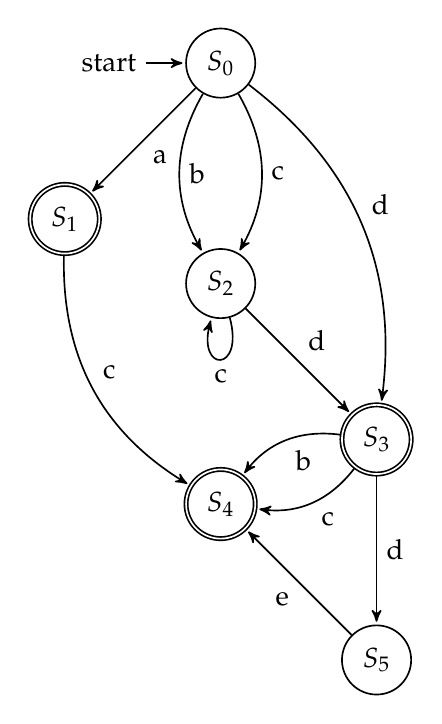
\begin{tikzpicture}[->, >=stealth', shorten >=1pt, auto, node distance=2.8cm,
                    semithick]
    \tikzstyle{every state}=[fill=none, text=black]

    \node[initial, state]   (A)                     {$S_0$};
    \node[state, accepting] (B) [below left of=A]   {$S_1$};
    \node[state]            (C) [below of=A]        {$S_2$};
    \node[state, accepting] (D) [below right of=C]  {$S_3$};
    \node[state, accepting] (E) [below of=C]        {$S_4$};
    \node[state]            (F) [below of=D]        {$S_5$};

    \path (A) edge                  node {a}            (B);
    \path (A) edge [bend right]     node {b}            (C);
    \path (A) edge [bend left]      node {c}            (C);
    \path (A) edge [bend left]      node {d}            (D);
    \path (C) edge [loop below]     node {c}            (C);
    \path (C) edge                  node {d}            (D);
    \path (B) edge [bend right]     node {c}            (E);
    \path (D) edge [bend right]     node {b}            (E);
    \path (D) edge [bend left]      node {c}            (E);
    \path (D) edge                  node {d}            (F);
    \path (F) edge                  node {e}            (E);
\end{tikzpicture}
\caption{Step 4: The full DFA with relabeled states.} \label{fig:prob2-step4}
\end{figure}

\newpage


\section{Problem 3}

\subsection{Ascending sequence of even numbers}

The language should consist of all strings of digits that contain all the even digits in ascending order as a subsequence.


\begin{equation}
\begin{split}
    R_a = \texttt{([0-9]*)0([0-9]*)2([0-9]*)} \\
          \texttt{4([0-9]*)6([0-9])8([0-9]*)}
\end{split}
\end{equation}


This regular expression accepts all strings of digits containing \texttt{02468} as a subsequence. The \texttt{[0-9]*} subexpressions interspersed among the sequence of even digits capture any digits that do not conform to the even, ascending subsequence. This will work under the assumption that the strings in the language can contain more even numbers than those forming the subsequence.


\subsection{No 011 subsequence}

\begin{equation}
\begin{split}
    R_b = \texttt{(1*)(0*)1?(0*)}
\end{split}
\end{equation}

This expression will accept any string of zeroes and ones for which \texttt{011} is not a subsequence, including the empty string.
By allowing only a single 1 after having captured a sequence of one or more \textit{0}s, we ensure that no \texttt{011} subsequence can occur.

\subsection{No 011 substring}

\begin{equation}
\begin{split}
    R_b = \texttt{(1*(0+1?)*)}
\end{split}
\end{equation}

$R_b$ allows zero or more leading \textit{1}s, but as soon as a zero is encountered, only two options are accepted;
more \textit{0}s until the string is terminated, or groups of one or more \textit{0}s and a single 1. It also allows the empty string.

\section{Problem 4}

\subsection{$n$ \textit{a}s followed by $n$ \textit{b}s, where $n > 1$}

As this is not a regular language, it is impossible to express using regular expressions. We need a context free grammar to express the production rules for this language. (E.g.: $S \rightarrow aSb$)

\subsection{$n$ \textit{a}s followed by $n$ \textit{b}s, where $n > 1$ and $n < 100$}

This, however, would work, as we could enumerate every possible production.


\subsection{Valid C99 source code}

No. Valid C source code allows for arbitrarily deep nesting of blocks.
A finite automaton has no memory outside of the state it is in.
To ensure the nesting is balanced, for source code of arbitrary length, we would need an arbitrarily large automaton.
This counters the notion of a \textit{finite} automaton, and expressing the language using regular expressions is therefore impossible.

\subsection{Valid C99 source code with a maximum length of 1000 characters}

Setting an upper limit on the length of the input gives us a finite amount of combinations. This means we can construct a \textit{finite} automata for the language and therefore altso a regular expression.

\end{multicols}

\end{document}
